\chapter{Introduction}
\label{chap:intro}

\section{Motivation}
\label{sect:motivation}
LiDAR senors provide critical depth information for autonomous driving and robotics. The LiDAR intensity maps are often spares and incomplete. Using depht maps as an addtional input is a way to impove the richness and accuracy ot the LiDAR predection. The Pix2Pix network for image-to-image translation offers a promising approch for integrating these modalities. 
\section{Contribution}
This project explores the use of the Pix2Pix network to predict LiDAR intensity maps by leveraging RGB images and depth maps as additional inputs.
\section{Related Work}
DeptAnything Models: \newline DepthAnything represents a significant advancement in monocular depth estimation by leveraging both labeled and unlabeled data at a large scale. Trained on 1.5 million labeled images and over 62 million unlabeled images, DepthAnything achieves state-of-the-art performance in depth estimation tasks. The model excels in both zero-shot relative and metric depth estimation, outperforming previous models such as MiDaS v3.1 and ZoeDepth. 
\newline
version 2
\newline
3D Reconstruction Techniques: 3D reconstruction is a broad field focused on creating three-dimensional models from two-dimensional images or depth data. Techniques in 3D reconstruction include methods like structure-from-motion (SfM), multi-view stereo (MVS), and volumetric approaches. These techniques aim to generate accurate 3D representations of scenes or objects from multiple views or depth sensors.

\chapter{Preparations}
used google colab, pix2pix network getting the right input, pix2pix problems



\chapter{Predicting LIDAR Intensity} %from RGB and Depth Images}
\section{Setup}
%The networks  net it is for depth completion and depth prediction
%pix2pix model with modified data loader to get 4 dim. input rgb plus depth
%used base model for depthanything
%The setup for this project involved configuring a series of models and datasets to predict LIDAR intensity from RGB and depth images. The key components and their roles are outlined below:
First of all the depth was created thru rgb pictures taken from "The KITTI Dataset". In order to get a great variatyof depth for comparison Bilateral Propagation Network (BP Net), Depthanything v1 \& 2 and metric v2 was used. The metric depth v1 was not used because it did not run intime.
\subsection{Bilateral Propagation Network (BP Net)}
\begin{itemize}
	\item \textbf{Purpose:} Used for depth completion to improve depth maps from incomplete or noisy data.
	\item \textbf{Dataset:} The input were raw data from kitti with a depth completion set already availible. 
\end{itemize}

\subsection{Depth Anything Models}
\begin{itemize}
	\item \textbf{Depth Anything v1:} Provided initial depth estimations using large-scale unlabeled data for zero-shot learning.
	\item \textbf{Depth Anything v2:} Enhanced depth prediction capabilities, incorporating improvements over v1 for better depth map accuracy.


 	\item \textbf {Metric Depth Estimation v2:} Supplemented depth maps with precise metric depth measurements.

	\item \textbf{Dataset:} Corresponding RGB images used in BP Net for better comparison.
\end{itemize}

\subsection{Pix2pix Network}
\begin{itemize}
	\item \textbf{Purpose:} Image to Image processing to predict LIDAR intensity from RGB and depth images.
	\item \textbf{Training Data:} RGB and depth pairs from the KITTI dataset.
	Eight different input data variations were used see in Chapter \ref{results}.
\end{itemize}

\section{Implementation}
\subsection{Depth Map Generation}
\begin{itemize}
	\item \textbf{BP Net:} An existing pretrained model on kitti data was loaded. Utilized BP Net and Depth Anything models to generate depth maps from the KITTI dataset. Depth maps were processed to ensure consistency and accuracy before use. The output was 1000 depthmaps
	
	\item \textbf{Depthaynthing v1 \& 2 and Metric Depth:} The depthaynthing networks provide also trained models for kitti. For all depthanything networks there aret three version availible. The smallm, base and large model. For similiar results the basemodel was loaded in each case.   
	
	\item \textbf{Dataset Preparation:} RGB images were paired with the generated depth maps to create a comprehensive training dataset for the pix2pix model.
	\end{itemize}
\begin{figure}[!ht]
	\centering
	%\scalebox{2}[1]{\includegraphics[width=0.2\textwidth]{abb/rgb/0000000030.png}}
	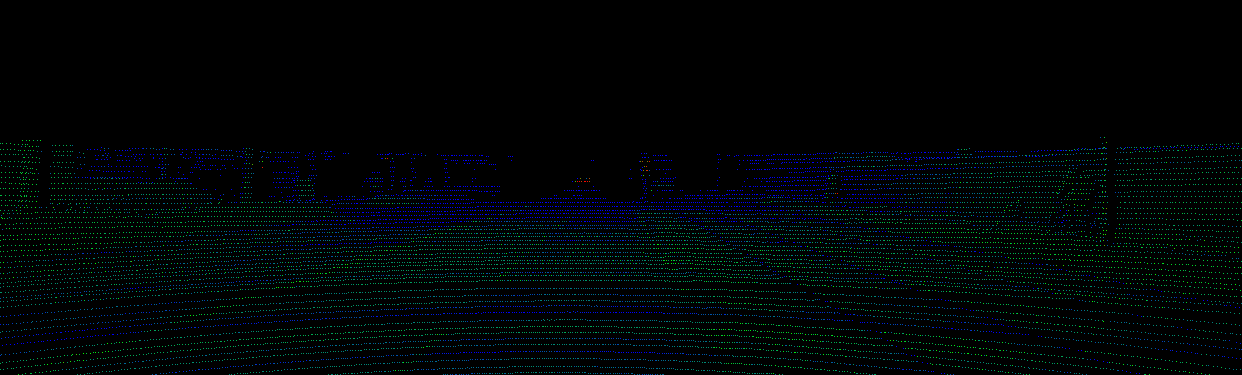
\includegraphics[width=0.5\textwidth]{abb/network/0000000077.png}
	\includegraphics[width=0.5\textwidth]{abb/network/0000000077bp.png}
	\includegraphics[width=0.5\textwidth]{abb/network/0000000077v1.png}
	\includegraphics[width=0.5\textwidth]{abb/network/0000000077v2.png}
	\includegraphics[width=0.5\textwidth]{abb/network/0000000077metric.png}
	\caption{RGB and created depth (BP, Deptanything v1,2 and metric v2)}
	\label{all_depths}
\end{figure}
The three dephtmaps sources (shown in picture \ref{all_depths}) have different properties. The BP Net has very little resultion in the nearfield. The depthanything depthmaps are both more dense in the nearfield but the far distant objects in backround are missing. The version 2 has better edge visualations and some distance objects like the sign on the lefthand side or the car are better visibel. The metric depth has the best focus on the farplane from all of them but near field has very little informtion. 

\newpage
\subsection{Model Training}\label{modeltraining}
\begin{itemize}
	\item \textbf{pix2pix Configuration:} The pix2pix architecture was adapted to accept RGB images and depth maps (4 dim.) as inputs to be able to scan input channel seperately and to avoid loss by overlaying rgb and depth images. The unmodified pix2pix was trained to predict LIDAR intensity values based on depthmaps inputs. The 4 dimensional pix2pix was given the input of rgb plus depthmaps.
	\item \textbf{Training Process:} The training parameters such as learning rate 0.0002000, batch size 1, and number of epochs 20 were set. The model was trained using the prepared dataset in the configuration 1000 pictures divided in 800 train, 100 val, 100 test folders. The input is differnet for the sole depth input and the rgbd input due to not equal running scripts for dividing. This was discoverd after the training and testing runs. Both versions were executed with masking out the pixel value -1 to reduce the areas which are not of interest. The input was crop to a size of 256 time 256  but not scale.
\end{itemize}

\section{Results} \label{results}
% wandb didnt work so no loss curves availble

%\newline
This section presents the results of the  experiments using different setups to predict LIDAR intensity. It was  evaluated the performance of several methods, including the seperate depths from BP Net, Depth Anything v1 and v2, as well as metric depth estimation to LiDAR. The other four are RGB plus each of these depths to LIDAR. The returning pictures are crop and the full verions a used as comparison. The crop version is the right part of the full resolution ($1216 \times 352$) images. For the 4 dimensional runs the cropped LiDAR groundtruth for better visualsation because this pix2pix version gives these extra outputs. The results from eight runs are summarized below:
%\newpage
\subsection{Depth BP Net to LIDAR}

Using only the depth maps generated by BP Net (Figure \ref{bp_results}), without accompanying RGB images, the model was trained to predict LIDAR intensity. This approach yielded shows some visible prediction.
\begin{figure}[!ht]
	\centering
	%\scalebox{2}[1]{\includegraphics[width=0.2\textwidth]{abb/rgb/0000000030.png}}
	\includegraphics[width=0.5\textwidth]{abb/singleruns/bp/depth/0000000070.png}
	\includegraphics[width=0.5\textwidth]{abb/singleruns/bp/lidar/0000000070.png}
	\includegraphics[width=0.5\textwidth]{abb/singleruns/bp/result/0000000070.png}
	\caption{RGB LiDAR and predicted LiDAR.}
	\label{bp_results}
\end{figure}
\newpage
\subsection{Depth Anything v1 to LIDAR}

The Depth Anything v1 model (Figure \ref{v1_results}) provided initial depth estimations using large-scale unlabeled data. When used to predict LIDAR intensity, this model showed results that are more familiar with depth maps and not LiDAR intensity.
\begin{figure}[!ht]
	\centering
	%\scalebox{2}[1]{\includegraphics[width=0.2\textwidth]{abb/rgb/0000000030.png}}
	\includegraphics[width=0.5\textwidth]{abb/singleruns/v1/depth/0000000070.png}
	\includegraphics[width=0.5\textwidth]{abb/singleruns/v1/lidar/0000000070.png}
	\includegraphics[width=0.5\textwidth]{abb/singleruns/v1/result/0000000070_depth.png}
	\caption{RGB LiDAR and predicted LiDAR.}
	\label{v1_results}
\end{figure}
\newpage
\subsection{Depth Anything v2 to LIDAR}

The Depth Anything v2 (Figure \ref{v2_results}) shows almost the same result like v1. It could be possible that pix2pix tried to learn LiDAR to depth but the datasets and the training settings were correct for that.
\begin{figure}[!ht]
	\centering
	%\scalebox{2}[1]{\includegraphics[width=0.2\textwidth]{abb/rgb/0000000030.png}}
	\includegraphics[width=0.5\textwidth]{abb/singleruns/v2/depth/0000000070.png}
	\includegraphics[width=0.5\textwidth]{abb/singleruns/v2/lidar/0000000070.png}
	\includegraphics[width=0.5\textwidth]{abb/singleruns/v2/result/0000000070.png}
	\caption{Depthanything v2 LiDAR and predicted LiDAR.}
	\label{v2_results}
\end{figure}
\newpage
\subsection{Metric Depth to LIDAR}

In this approach, precise metric depth measurements (Figure \ref{metric_results}) were used to predict LIDAR intensity. This method significantly shows some good prediction of the LiDAR intensity.
\begin{figure}[!ht]
	\centering
	%\scalebox{2}[1]{\includegraphics[width=0.2\textwidth]{abb/rgb/0000000030.png}}
	\includegraphics[width=0.5\textwidth]{abb/singleruns/metricv2/depth/0000000070.png}
	\includegraphics[width=0.5\textwidth]{abb/singleruns/metricv2/lidar/0000000070.png}
	\includegraphics[width=0.5\textwidth]{abb/singleruns/metricv2/result/0000000070.png}
	\caption{Metricdepth LiDAR and predicted LiDAR.}
	\label{metric_results}
\end{figure}
\newpage	
\subsection{RGB plus BP Net to LIDAR}
In this setup (Figure \ref{bp_rgbd}), RGB images were combined with depth maps generated by the BP Net model to predict LIDAR intensity. The integration of depth information from BP Net significantly displayes some correct prediction accuracy compared to using Depth maps images alone. The cars for instance are barely visibile and the backround is almost filled wrong perhaps due to the masking.
\begin{figure}[!ht]
	\centering
	% Erstes Bild
	\begin{subfigure}{0.4\textwidth}
		\centering
		\includegraphics[width=\linewidth]{abb/plusdepthruns/bp/rgb/0000000069.png}
		\caption{RGB Image}
		\label{bp_rgbd1}
	\end{subfigure}
	
	\vspace{1em} % Vertikaler Abstand zwischen den Bildern
	
	% Zweites Bild
	\begin{subfigure}{0.4\textwidth}
		\centering
		\includegraphics[width=\linewidth]{abb/plusdepthruns/bp/depth/0000000069.png}
		\caption{Depth Map}
		\label{bp_rgbd2}
	\end{subfigure}
	
	\vspace{1em} % Vertikaler Abstand zwischen den oberen und unteren Bildern
	
	% Drittes und viertes Bild nebeneinander
	\begin{subfigure}{0.25\textwidth}
		\centering
		\includegraphics[width=\linewidth]{abb/plusdepthruns/bp/result/0000000069_real_B.png}
		\caption{Groundtruth LiDAR}
		\label{fig:bp_pred_lidar}
	\end{subfigure}
	%hfill
	\begin{subfigure}{0.25\textwidth}
		\centering
		\includegraphics[width=\linewidth]{abb/plusdepthruns/bp/result/0000000069_fake_B.png}
		\caption{Predicted LiDAR}
		\label{fig:bp_fake_lidar}
	\end{subfigure}
	
	\caption{RGB, Depth, Predicted LiDAR, and Predicted LiDAR images for the BP Net setup.}
	\label{bp_rgbd}
\end{figure}
\newpage
\subsection{RGB plus Depth Anything v1 to LIDAR}
Combining RGB images with depth maps from Depth Anything v1 (Figure \ref{v1_rgbd}), the model achieved better performance than using depth alone. The fusion of RGB and depth data provided a more comprehensive input, resulting in an LIDAR intensity but it show little reselemblest to the groundtruth.
\begin{figure}[!ht]
	\centering
	% Erstes Bild
	\begin{subfigure}{0.4\textwidth}
		\centering
		\includegraphics[width=\linewidth]{abb/plusdepthruns/v1/rgb/0000000070.png}
		\caption{RGB Image}
		\label{fig:v1_rgb}
	\end{subfigure}
	
	\vspace{1em} % Vertikaler Abstand zwischen den Bildern
	
	% Zweites Bild
	\begin{subfigure}{0.4\textwidth}
		\centering
		\includegraphics[width=\linewidth]{abb/plusdepthruns/v1/depth/0000000070.png}
		\caption{Depth Map}
		\label{fig:v1_depth}
	\end{subfigure}
	
	\vspace{1em} % Vertikaler Abstand zwischen den oberen und unteren Bildern
	
	% Drittes und viertes Bild nebeneinander
	\begin{subfigure}{0.25\textwidth}
		\centering
		\includegraphics[width=\linewidth]{abb/plusdepthruns/v1/result/0000000070_real_B.png}
		\caption{Groundtruth LiDAR}
		\label{fig:v1_pred_lidar}
	\end{subfigure}
	%hfill
	\begin{subfigure}{0.25\textwidth}
		\centering
		\includegraphics[width=\linewidth]{abb/plusdepthruns/v1/result/0000000070_fake_B.png}
		\caption{Predicted LiDAR}
		\label{fig:v1_fake_lidar}
	\end{subfigure}
	
	\caption{RGB, Depth, Predicted LiDAR, and Predicted LiDAR images for the Depth Anything v1 setup.}
	\label{v1_rgbd}
\end{figure}
\newpage
\subsection{RGB plus Depth Anything v2 to LIDAR}
RGB images paired with depth maps from Depth Anything v2 (Figure \ref{v2_results}) show a better predection than v1. The sign in the groundtruth is more visible due to better depthmaps resolution of the depthanything v2.
\begin{figure}[!ht]
	\centering
	% Erstes Bild
	\begin{subfigure}{0.4\textwidth}
		\centering
		\includegraphics[width=\linewidth]{abb/plusdepthruns/v2/rgb/0000000070.png}
		\caption{RGB Image}
		\label{fig:v2_rgb}
	\end{subfigure}
	
	\vspace{1em} % Vertikaler Abstand zwischen den Bildern
	
	% Zweites Bild
	\begin{subfigure}{0.4\textwidth}
		\centering
		\includegraphics[width=\linewidth]{abb/plusdepthruns/v2/depth/0000000070.png}
		\caption{Depth Map}
		\label{fig:v2_depth}
	\end{subfigure}
	
	\vspace{1em} % Vertikaler Abstand zwischen den oberen und unteren Bildern
	
	% Drittes und viertes Bild nebeneinander
	\begin{subfigure}{0.25\textwidth}
		\centering
		\includegraphics[width=\linewidth]{abb/plusdepthruns/v2/result/0000000070_real_B.png}
		\caption{Groundtruth LiDAR}
		\label{fig:v2_pred_lidar}
	\end{subfigure}
	%hfill
	\begin{subfigure}{0.25\textwidth}
		\centering
		\includegraphics[width=\linewidth]{abb/plusdepthruns/v2/result/0000000070_fake_B.png}
		\caption{Predicted LiDAR}
		\label{v2}
	\end{subfigure}
	
	\caption{RGB, Depth, Predicted LiDAR, and Predicted LiDAR images for the Depth Anything v2 setup.}
	\label{v2_rgbd}
\end{figure}
\subsection{RGB plus Metric Depth to LIDAR}

The combination of RGB images with precise metric (Figure \ref{metric_rgbd})depth measurements led to the most accurate predictions of LIDAR intensity. This setup utilized the strengths of both RGB data and metric depth, achieving the best results across all runs. The conturs of the cars on the right side are visible. 

\begin{figure}[!ht]
	\centering
	
	% Erstes Bild
	\begin{subfigure}{0.4\textwidth}
		\centering
		\includegraphics[width=\linewidth]{abb/plusdepthruns/metricv2/rgb/0000000417.png}
		\caption{RGB}
		\label{fig:bild1}
	\end{subfigure}
	
	\vspace{1em} % Vertikaler Abstand zwischen den Bildern
	
	% Zweites Bild
	\begin{subfigure}{0.4\textwidth}
		\centering
		\includegraphics[width=\linewidth]{abb/plusdepthruns/metricv2/depth/0000000417.png}
		\caption{Depth}
		\label{fig:bild2}
	\end{subfigure}
	
	\vspace{1em} % Vertikaler Abstand zwischen den oberen und unteren Bildern
	
	% Drittes und viertes Bild nebeneinander
	\begin{subfigure}{0.25\textwidth}
		\centering
		\includegraphics[width=\linewidth]{abb/plusdepthruns/metricv2/result/0000000417_real_B.png}
		\caption{Groundtruth LiDAR}
		\label{fig:bild3}
	\end{subfigure}
	%%hfill
	\begin{subfigure}{0.25\textwidth}
		\centering
		\includegraphics[width=\linewidth]{abb/plusdepthruns/metricv2/result/0000000417_fake_B.png}
		\caption{Predicted LiDAR}
		\label{fig:bild4}
	\end{subfigure}
	
	\caption{RGB Depthanything metric LiDAR and predicted LiDAR.}
	\label{metric_rgbd}
\end{figure}
\chapter{Conclusion}
The approches with the rgb and depth only result in bad prediction. the bp 

\section{Appendix}
\subsection{RGB to LIDAR}

The model trained using only RGB images to predict LIDAR intensity was evaluated. RGB alone provided sparse level of prediction, it lacked the accuracy required for high-precision applications. ere is a citation for the Depth Anything paper \cite{depthanything}, its version 2 \cite{depth_anything_v2}, and for the paper by Saxena et al. \cite{saxena2008depth}
\begin{figure}[!ht]
	\centering
	%\scalebox{2}[1]{\includegraphics[width=0.2\textwidth]{abb/rgb/0000000030.png}}
	\includegraphics[width=0.3\textwidth]{abb/singleruns/rgb/rgb/0000000070.png}
	\includegraphics[width=0.3\textwidth]{abb/singleruns/rgb/lidar/0000000030.png}
	\scalebox{2}[0.5]{\includegraphics[width=0.3\textwidth]{abb/singleruns/rgb/result/0000000070.png}}
	\caption{RGB LiDAR and predicted LiDAR.}
	\label{rgb}
\end{figure}


\section{References}
bp net work
pix2pix
depth anything v1 2
paper for them 
some for lidar intensity
